\chapter{Introduction}
\label{chap:intro}

\section{Charge Transport in Organic Semiconductors}
\subsection{Organic Semiconductors}
Conductive polymers were first discovered in 1977 by Shirakawa et al  \cite{chiang_electrical_1977, Shirakawa1977Jan} for which they were awarded the Nobel prize in Chemistry. Since then, these materials have become widespread in many technologies, such as in organic photovoltaic cells\cite{Kippelen2009}, organic field-effect transistors (OFET) \cite{Malachowski2010Jun} and organic light-emitting diodes (OLED) \cite{ThejoKalyani2012Jun}. While the other two technologies lag behind their inorganic counterparts, uptake of OLED screens is becoming ubiquitous -especially in the smartphone and television market due to their flexibility, better colour representation and lower energy consumption than standard backlit LCD displays. OLEDs have also found uses in lighting with their efficiency rivalling that of fluorescent tubes \cite{Reineke2009May, OLED_lighting}. Although, industry has made large strides in fabricating and using these materials the exact nature of the charge transport is still poorly understood. Traditional theories (such as hopping and band transport) aren't applicable to many relevant materials \cite{coropceanu_charge_2007, Giannini2019, C0CS00198H, Fratini_2016, yavuz_dichotomy_2017} as charge transfer dynamics lies in an intermediate region where the charge carrier forms a polaron which is neither fully localised or delocalised. In organic semiconductors, typical values of the localisation of the polaron are between 2 $\rightarrow$ 20 molecules. This is due to crystals typically being formed of organic molecules weakly held together by Van der Waals (VDW) forces rather than strong covalent bonds. This allows molecules to fluctuate about their lattice sites and introduces larger quantities of (dynamic) disorder than is present in inorganic crystals. 
\\\\
There are a number of techniques currently used in the field to evaluate the performance of organic semiconductors, though all come with their own caveats. For example, transient localisation theory (TLT) \cite{Nematiaram2019, PhysRevB.83.081202, Fratini_2016}, while efficient and accurate, cannot be used in non-periodic systems or those with large amounts of static disorder. Another technique, multi-configurational time-dependent Hartree (MCTDH) \cite{MCTDH, cattarius_all_2001}, is considered the gold standard for wavepacket propagation and has been used extensively in numerous studies (e.g. refs \cite{MANTHE19937,doi:10.1063/1.463332,doi:10.1063/1.469292}). However, due to the treatment of the full system  (including nuclei) quantum mechanically, MCTDH is relatively expensive and can only be applied to a small molecular systems. In this work I will be studying electron-nuclear propagation methods that rely on the treatment of the nuclear degrees of freedom classically and the electronic ones quantum mechanically. This is approximation is termed the semi-classical approximation and allows the efficient simulation of mesoscopic systems.
\\\\
There are a number of semi-classical techniques used in the field. The most common are fewest switches surface hopping (FSSH) \cite{FSSH_orig} and mean-field dynamics (also called Ehrenfest dynamics) \cite{Ehrenfest1927}. In addition to these, in this work I will be exploring a relative newcomer to the (nonadiabatic) semi-classical simulation arsenal, namely coupled-trajectory mixed quantum-classical molecular dynamics (CTMQC). I will be focussed on the extension of these algorithms and their application to organic semiconducting systems, containing a hundreds of molecules.

\section{Semi-classical Nonadiabatic Molecular Dynamics}
Semi-classical techniques all decompose the nuclear and electronic degrees of freedom and propagate nuclei with Newton's equations using standard molecular dynamics \cite{Coker1995Jan}. Here the forces are calculated with a parameterised forcefield and positions and velocities are often updated with the velocity Verlet technique. The forcefield outlines the shape of the potential energy surface (PES) the nuclei evolve on. The electronic subsystem is propagated using a variety of techniques that solve the time-dependent Schr\"odinger equation. There are numerous techniques for the calculating electronic properties used in propagation, though the most common are density functional theory (DFT) and model Hamiltonian based methods. However, in nonadiabatic processes (such as in charge transfer \cite{PhysRevB.79.115203} or photoexcitation \cite{Hammes-Schiffer2001Apr, Hammes-Schiffer1994Sep, Huynh2007}) the nuclear and electronic subsystems are not independent. That is, the specific nuclear geometry depends on the electron density and vice-versa. The resulting interaction between these 2 subsystems is the way each of the semi-classical techniques differ. In this regime the Born-Oppenheimer approximation cannot be applied \cite{john_c._tully_nonadiabatic_nodate}. This approximation, relied upon for almost a century \cite{Pisana2007Feb}, hinges on the fact that nuclei are much more massive than electrons and are approximately stationary with respect to electron motion\cite{Born1927Jan}. This results in nuclear evolution that is governed by a single, adiabatic, potential energy surface. Nonadiabatic molecular dynamics methods, such as the aforementioned surface hopping and mean-field techniques, facilitates the bypassing of this limitation and can be used to simulate molecular dynamics with electronic transitions. 
\\\\
\subsection{Ehrenfest Dynamics}
\begin{figure}[htp]
  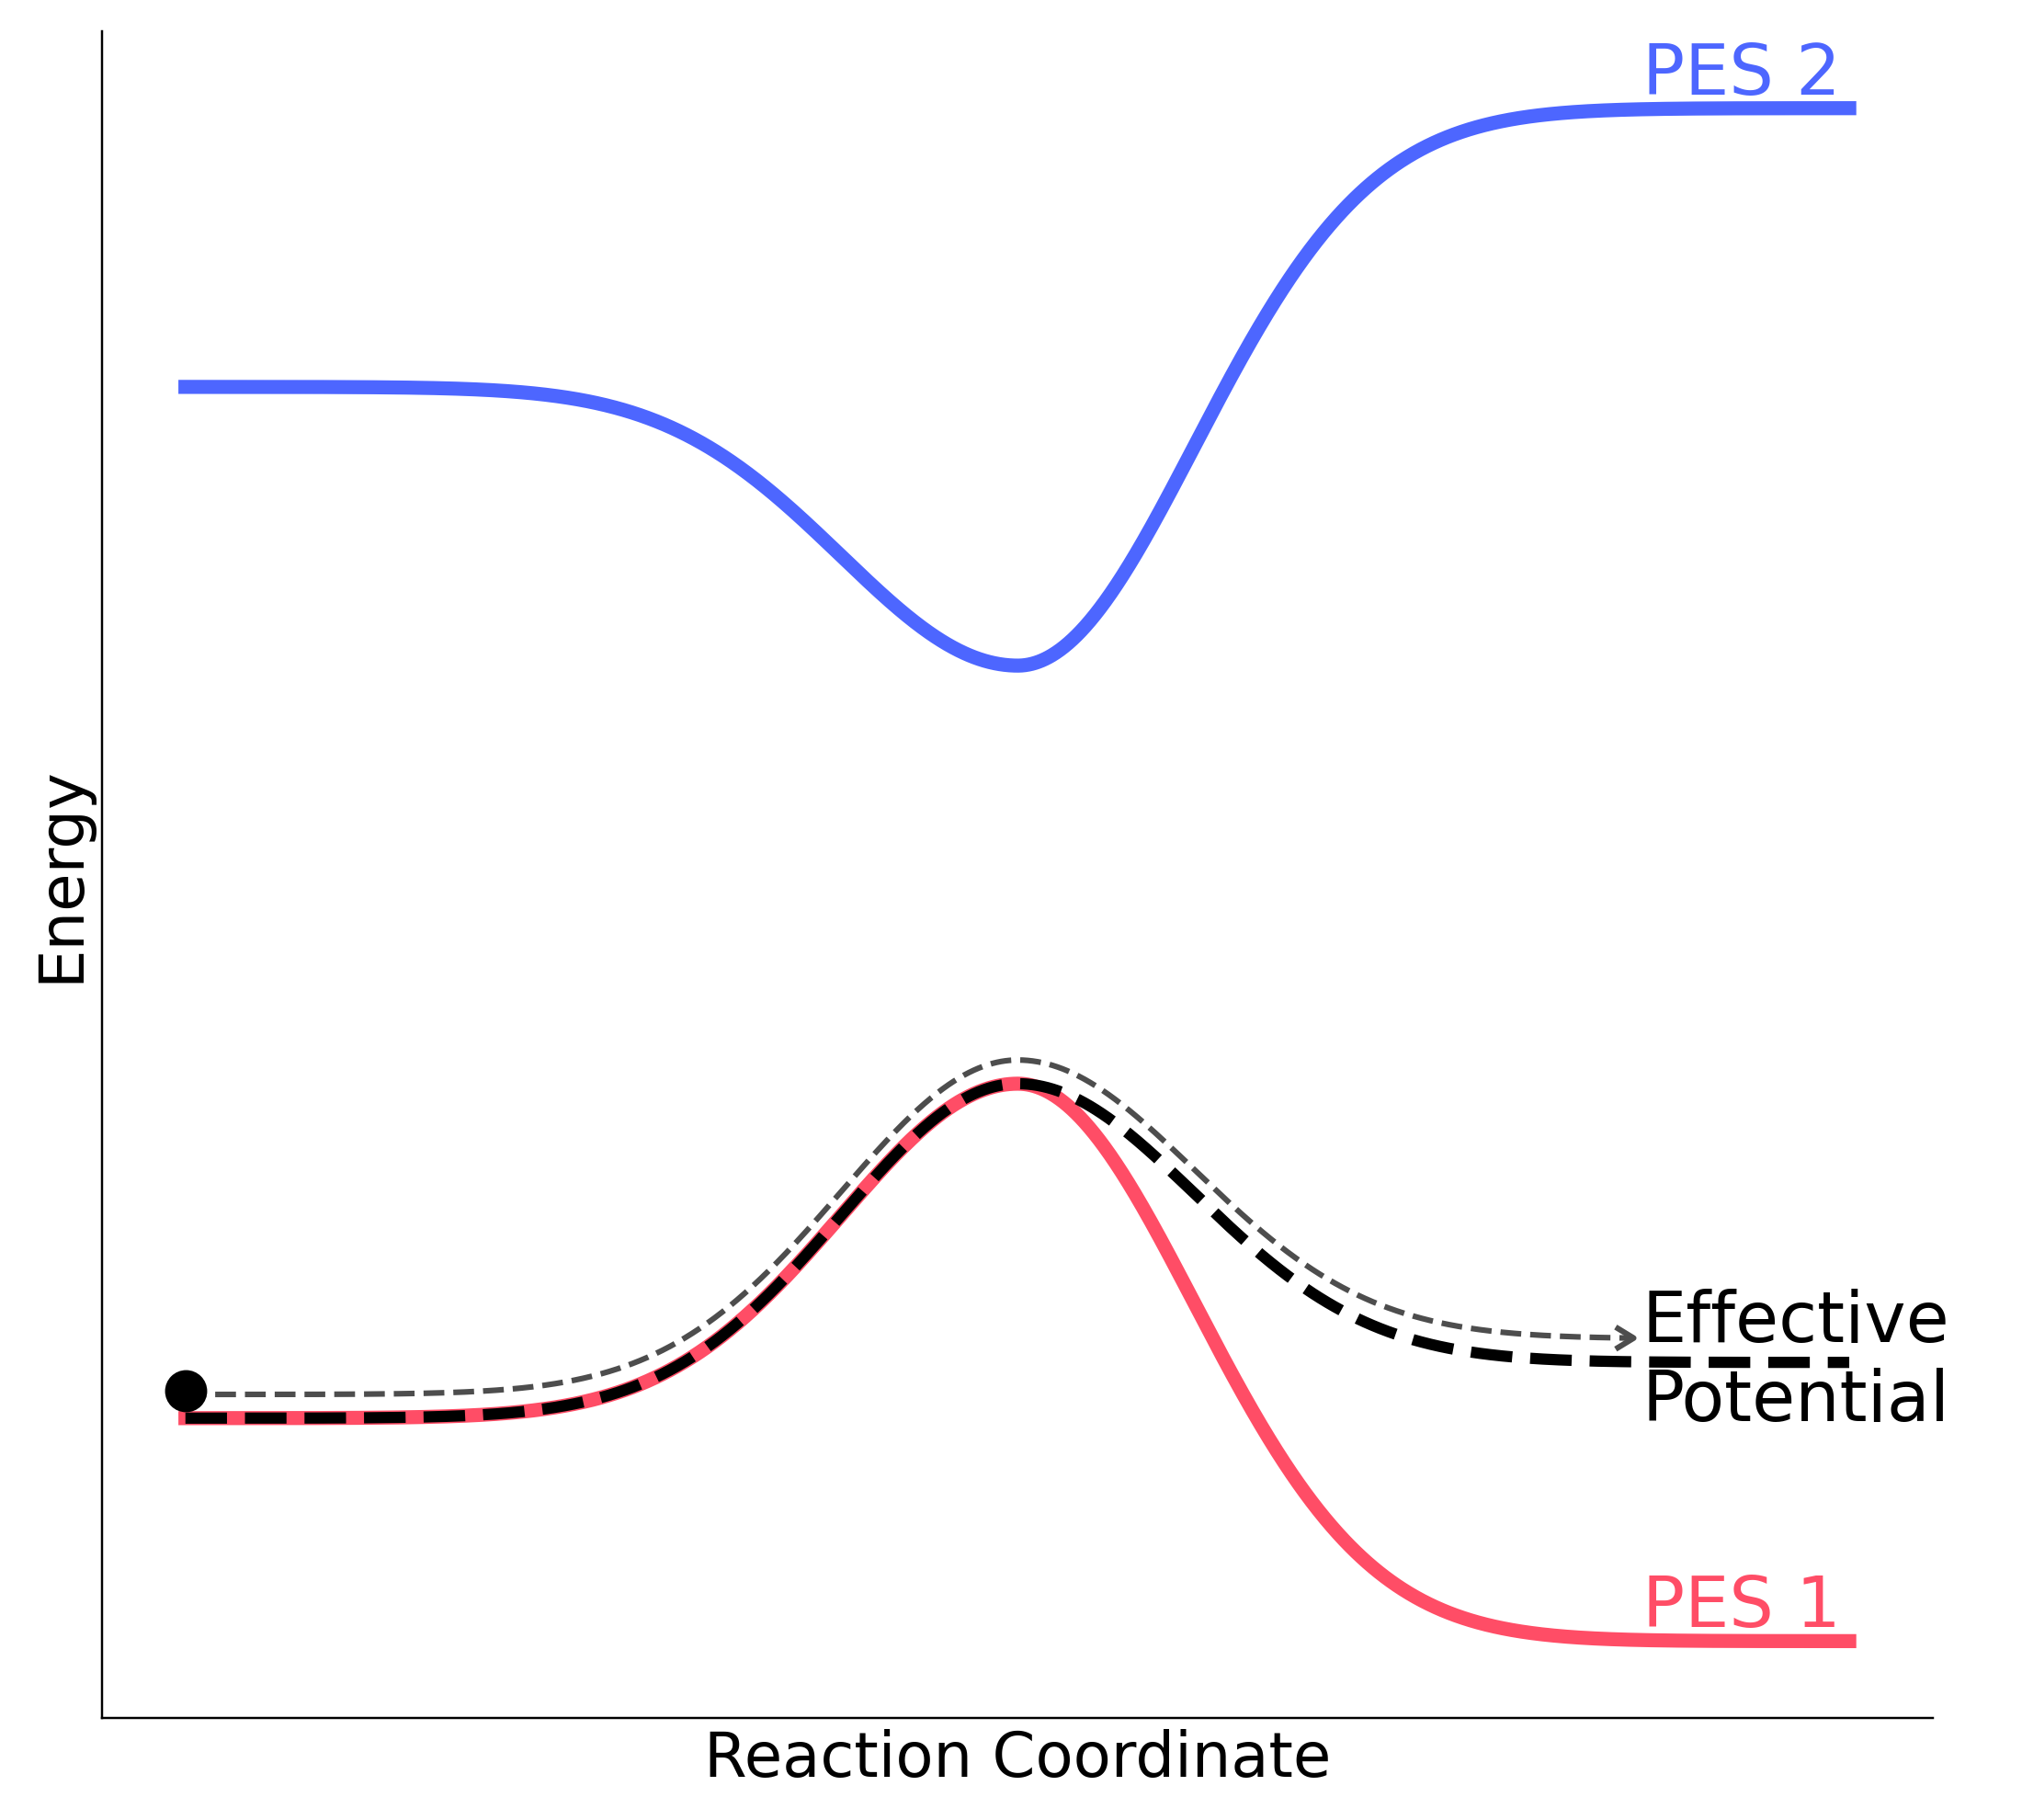
\includegraphics[width=\textwidth]{./img/Eh_hop.png}
  \caption{\label{fig:Eh_diag}An example of a typical Ehrenfest simulation near an avoided crossing. The black lines represent the adiabatic potential energy surface due to the ground (PES 1) and excited (PES 2) state. The red line represents the population weighted average potential the nuclei travel on.}
\end{figure}
\noindent The oldest, and most intuitive, NAMD method is Ehrenfest dynamics \cite{Ehren1927}. In this technique the nuclei evolve on a single, mean potential energy surface (PES). The shape of this PES comes from a population-weighted average, hence the electronic subsystem can influence the nuclear dynamics through the PES. This is method of propagation is displayed for a simple 1D, 1 atom, 2 state system in figure \ref{fig:Eh_diag}. In this figure we initialise the adiabatic population in the ground (red) state. As the atom (black dot) progress through the reaction coordinates it feels forces equal to the negative gradient of the population-weighted average PES (dotted black line).
\\\\
The Ehrenfest equations can be rigorously derived from the time-dependent Schr\"odinger equation by expanding the full the full electronic wavefunction as a linear combination of adiabatic states as in equation \eqref{eq:BornHuangExpansion} and assuming that the nuclei's motion is determined by a single population-weighted PES. The equation for the calculation of these forces is given in equation \eqref{eq:Eh_Force}.
\begin{equation}
  \Psi(\mathbf{r}, \mathbf{R}, t) = \sum_{m} C_{m}(\mathbf{R}, t) \phi_i(\mathbf{r}, t)
  \label{eq:BornHuangExpansion}
\end{equation}
Where the full electronic wavefunction $\Psi(\mathbf{r}, \mathbf{R}, t)$ is expanded as a sum of adiabatic expansion coefficients $C_{m}$ multiplied by an adiabatic basis function $\phi_i$. The norm of the adiabatic expansion coefficients gives the probability of finding the wavefunction in state $m$.
\begin{equation}
  \mathbf{F}_{\nu}^{Ehren} = \sum_i^{N_{st}} |C_{m}|^2 \mathbf{\nabla}_{\nu} E_{m} + \sum_{m \neq n}^{N_{st}} C_{m}^{*} C_{n} (E_{n} - E_{m}) \mathbf{d}_{ij, \nu}^{ad}
  \label{eq:Eh_Force}
\end{equation}
Where the force, $\mathbf{F}$, for each atom, $\nu$ is the sum of the adiabatic population, $|C_{m}|^2$, on each state, $m$, multiplied by the gradient of the adiabatic energy of state $\mathbf{\nabla}_{\nu}E_{m}$ plus the sum over pairs of adiabatic states, $m$ and $n$, of the adiabatic expansion coefficients, $C_{m (n)}$ multiplied by the energy difference $E_{n} - E_{m}$ multiplied by the nonadiabatic coupling vector $\mathbf{d}_{ij, \nu}$ on atom $\nu$. The adiabatic energies are calculated as the eigenvalues of the hamiltonian.
\\\\
The equation for the propagation of the adiabatic expansion coefficients is given in equation \eqref{eq:Eh_Elec}.
\begin{equation}
  \im \ \hbar \dot{C}_{m} = C_{m}E_{m} -  \im \ \hbar  \sum_{n}^{N_{st}} C_{n} \sum_{\nu} \mathbf{v}_{\nu} \cdot \mathbf{d}^{ad}_{mn, \nu}
  \label{eq:Eh_Elec}
\end{equation}
We can see in this equation any mixing of electronic population between states is initially stimulated by the dot between the nonadiabatic coupling vector and the nuclear velocity, $\sum_{\nu} \mathbf{v}_{\nu} \cdot \mathbf{d}_{nm, \nu}^{ad}$. In figure \ref{fig:Eh_diag} the coupling would be highest near the middle of the figure, where the 2 PES come the closest to each other, so populations would only start mixing when the nuclei reached this point. This, and the fact that the Hamiltonian (and therefore adiabatic energies) is a function of nuclear positions, is the method of feedback from the nuclear to the electronic subsystem. 
\\\\
Although the Ehrenfest method has been applied with success in many systems \cite{Li2005Aug, Saita2012Dec, Kohen1998Sep} it has a number of key shortcomings. Namely, its inability to capture the branching of the nuclear wavefunction (as propagation occurs on only a single PES) and its poor account of the decoherence of the electronic and nuclear subsystem after an avoided crossing. Ehrenfest also violates detailed balance and prevents the thermodynamic equilibration of the system by populating all adiabatic states evenly \cite{tully_perspective:_2012, john_c._tully_nonadiabatic_nodate}. In the limit of infinite states this results in infinite electronic temperature \cite{parandekar_detailed_2006}. For this reason many people choose to use fewest switches surface hopping.

\subsection{Surface hopping}
\begin{figure}[htp]
  \includegraphics[width=\textwidth]{./img/SH_hop.png}
  \caption{\label{fig:SH_diag}An example of a typical Surface Hopping simulation near an avoided crossing. The black lines represent the adiabatic potential energy surface due to the ground (PES 1) and excited (PES 2) state. The red line represents the discontinuous effective potential the nuclei travel on.}
\end{figure}
Surface hopping was devised to circumvent the limitations of mean-field NAMD. To do this a swarm of trajectories is initialised and allowed to propagate independently throughout the system. These trajectories represent the nuclear wavepacket and can have varied paths depending on the topology of the system. The shape of the PES on each trajectory is determined by discrete, stochastic hops between adiabatic potential energy surfaces. This is demonstrated for a single trajectory in figure \ref{fig:SH_diag}. In this cartoon, the expansion coefficient is initialised with its population on the ground (red) state. As the atom travels towards the avoided crossing (region of high nonadiabatic coupling), the likelihood of a hop increases. A random number is used to decide whether the hop occurs, if it does the velocities of the nuclei are adjusted/rescaled to account for the energy difference in PES (along the direction of the NACV). This is shown towards the center of figure \ref{fig:SH_diag}. After the atom has hopped to the upper surface it experiences forces equivalent to the negative gradient of the PES. In this situation it results in the atom begin reflected at the avoided crossing. Some trajectories will hop here and some won't (depending on the coupling strength) resulting in a branching of the nuclear wavepacket. This is in contrast to Ehrenfest, where all trajectories travel along the same PES, meaning the nuclear wavepacket cannot branch.
\\\\
The propagation of the adiabatic expansion coefficients is the same as for Ehrenfest and is given in equation \eqref{eq:Eh_Elec}. This results in 2 forms of adiabatic populations, the surface population (the fraction of trajectories on each PES) and the adiabatic population (the population of the adiabatic expansion coefficients). These 2 populations should agree and when they do the system is said to obey internal consistency. The forces are given by the negative gradient of the potential energy surface the trajectory is travelling on. This is given in equation \eqref{eq:SH_force}
\begin{equation}
  \mathbf{F}_{\nu} = -\mathbf{\nabla}_{\nu} E_{i} 
  \label{eq:SH_force}
\end{equation}
Where the force on atom $\nu$ is equal to the gradient (with respect to atom $\nu$) of potential energy surface $i$.
\\\\
Although surface hopping fixes many concerns from Ehrenfest dynamics there are still caveats to be aware of. The original `fewest switches surface hopping' proposed by John Tully suffered from bad overcoherence of the nuclear and electronic subsystems. That is the electronic and nuclear motion was coupled long after the region of high non-adiabatic coupling (crossing region). There have been attempts to fix this by introducing a decoherence time, after which the adiabatic population is forced to occupy a single state (either instantly or exponentially damped). However, the parameterisation of this time isn't trivial and many methods have been proposed. A decoherence method where non active adiabatic populations are exponentially damped and the active state is adjusted to conserve the norm is used in this work. The damping time is based on Heisenberg uncertainty principle and the energy difference between the active state and the inactive states. Full details of this method are given in refs \cite{Giannini2018Crossover, Carof2017FSSH}.
\\\\
Further deficiencies of trajectory surface hopping are the fact that the hops are instant which can lead to discontinuities in the total energy. The standard methods to compensate for this is re-scaling velocities along the direction of the NACV (as mentioned previously). Due to the nuclear timestep being finite trivial crossings can be missed with propagating the system. This is because when adiabatic states become very close to each other (or even totally degenerate) the nonadiabatic coupling can form a large, sharp peak with respect to the reaction coordinate. If the nuclear timestep is too large this large peak can be completely missed leading to several artifacts. There have been various solutions proposed that are referenced in ref \cite{Carof2017FSSH, Wang2016}. In this work, I will use the self-consistent surface hopping correction introduced by Wang and Prezhdo \cite{Wang2014}.  A final shortcoming of surface hopping is that it has not been derived from first principles and cannot be guaranteed to work generally. Though, in practise, surface hopping has been widely adopted and tested on a variety of systems and its suitability for use in these has been reported and many problems have been addressed \cite{Wang2016}.
\\\\
The ongoing search to address these issues, and ultimately develop the panacea of nonadiabatic molecular dynamics techniques, has lead to a number of other techniques being developed. One of these, CTMQC, will be studied in detail in this thesis and is the semi-classical limit of the exact factorisation of the time-dependent Schr\"odinger equation.
\section{Exact Factorisation and its Semi-Classical Limit}
Exact factorisation \cite{abedi_exact_2010} involves separating the total molecular wavefunction into a nuclear component and electronic component. Where the electronic component is parametrically dependent on the nuclear coordinates, $\mathbf{R}$. This is shown below in eq \eqref{eq:exact_fact} where $\chi$ is the nuclear wavefunction and $\Phi$ is the electronic one.
\begin{equation}
 \Psi(\mathbf{R}, \mathbf{r}, t) = \Phi_{\mathbf{R}}(\mathbf{r}, t) \chi(\mathbf{R}, t)
 \label{eq:exact_fact}
 \end{equation}
 In the above equation (and throughout this report) I will denote nuclear coordinates and electronic coordinates $\mathbf{R}$ and $\mathbf{r}$ respectively. The nuclear and electronic wavefunctions then obey separate, but coupled, time-dependent Schr\"odinger equations for spatial and temporal evolution. In this report, I will be focussing on the semi-classical limit of these equations, named Coupled-Trajectory Mixed Quantum-Classical Molecular Dynamics (CTMQC), and give results of a combination of this and the AOM method explained in appendix \ref{ap:AOM}.
\\\\
The equations for the evolution of the electronic and nuclear wavefunctions in the exact factorisation \cite{abedi_exact_2010} are given below:
\begin{align}
  \im\hbar \frac{\delta}{\delta t} \Phi_{\mathbf{R}}(\mathbf{r}, t) &= \left( \hat{H}_{BO} + \hat{U}_{en}\left[ \Phi_{\mathbf{R}}, \chi\right] - \epsilon(\mathbf{R}, t) \right) \Phi_{\mathbf{R}} (\mathbf{r}, t)
  \label{eq:electronic_exact}
\\
\im\hbar \frac{\delta}{\delta t} \chi (\mathbf{R}, t) &= \left( \sum_{\nu = 1}^{N_{n}} \frac{[-\im\hbar\nabla_{\nu} + \mathbf{A}_{\nu}(\mathbf{R}, t)]^2}{2 M_{\nu}} + \epsilon(\mathbf{R}, t)\right) \chi (\mathbf{R}, t)
  \label{eq:nuclear_exact}
\end{align}
Where $\hat{H}_{BO}$ is the Born-Oppenheimer Hamiltonian, that is $\hat{T}_{e} + \hat{W}_{ee} + \hat{W}_{nn} + \hat{V}_{en}$. Where $\hat{T}_{e}$ is the electronic kinetic energy operator, $\hat{W}_{ee/nn}$ is the electron-electron/nuclei-nuclei interaction and $V_{en}$ is the electronic-nuclear potential.
\\\\
The $\hat{U}_{en}$ is an electronic-nuclear coupling operator (ENCO). This is defined as \begin{equation}
  \hat{U}_{en}[\Phi_{\mathbf{R}}, \chi] = \sum_{\nu=1}^{N_{nuc}} \frac{1}{M_{\nu}} \left[ \frac{\left[-i \hbar \nabla_{\nu} - \mathbf{A}_{\nu}(\mathbf{R}, t) \right]^2}{2} + \left( \left. \left. \frac{-i\hbar \nabla_{\nu} \chi}{\chi} + \mathbf{A}_{\nu}(\mathbf{R, t})\right)\right( -i\hbar\nabla_{\nu} -            \mathbf{A}_{\nu}(\mathbf{R}, t)\right) \right]
  \label{eq:ENCO}
\end{equation}
\\
Where the $\mathbf{A}_{\nu}$ is a time-dependent vector potential (TDVP), given by $\left\langle \Phi_{\mathbf{R}}(t) \right\vert \left. - i \hbar \nabla_{\nu} \Phi_{\mathbf{R}} \right\rangle_{\mathbf{r}}$ and $M_{\nu}$ is the mass of nuclei $\nu$.
Finally $\epsilon(\mathbf{R}, t)$ is a time-dependent scalar potential energy surface (TDPES), given by $\langle \Phi_{\mathbf{R}}(t) \vert \hat{H}_{BO} + \hat{U}_{en}^{coup} - i\hbar \frac{\delta}{\delta t} \vert \Phi_{\mathbf{R}}(t) \rangle_{\mathbf{r}}$.
\\
\begin{figure}[htp]
  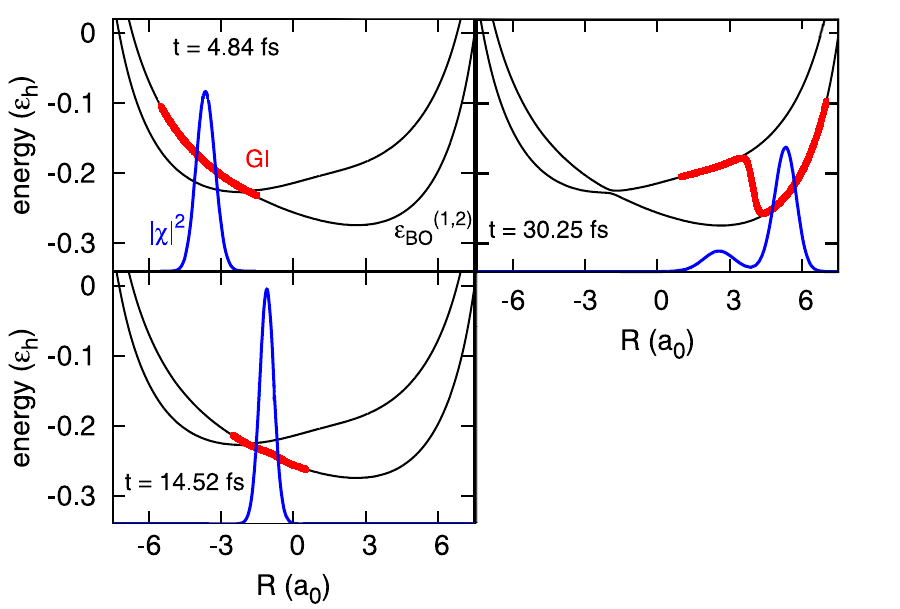
\includegraphics[width=\textwidth]{./img/CTMQC/nuclear_splitting_TDPES.png}
  \caption{A demonstration of how the TDPES can cause the splitting of the nuclear wavepacket in non-adiabatic regions. The red line represents the TDPES and the blue is the nuclear density. Figure adapted from Agostini, 15 \cite{agostini_exact_2015} \label{fig:step_TDPES}}
\end{figure}
\\
The effects of the TDPES, TDVP and the ENCO have been investigated in multiple works \cite{agostini_semiclassical_2015, agostini_exact_2015, agostini_mixed_2013, abedi_dynamical_2013, Min2014Dec}. The TDPES and TDVP are both responsible for the evolution of the system
\cite{agostini_semiclassical_2015}. The TDPES provides exact classical forces on the nuclei. In fact, an alternative independent-trajectory semi-classical scheme has been investigated using these exact forces \cite{agostini_exact_2015}. This found the TDPES is responsible for the splitting of the nuclear wavepacket in regions of high non-adiabaticity by taking the shape of a step function between the 2 adiabatic potentials. This is demonstrated in figure \ref{fig:step_TDPES}, which was adapted from an image in Agostini, 15 \cite{agostini_semiclassical_2015}. We can see the as the simulation progresses the initial nuclear density (blue curve) becomes split when the TDPES (red curve) forms a sharp step. This occurs just after the avoided crossing region. The 2 ends of the nuclear density then feel different forces from the 2 potential energy surfaces and evolve separately. Finally the electronic-nuclear coupling operator (ENCO) is responsible for other non-adiabatic effects in the system such as electronic nonadiabatic transitions and decoherence \cite{agostini_semiclassical_2015}.
\section{Approximations leading to CTMQC}
\label{sect:CTMQC_Approx}
Starting from the exact factorisation equations, 5 approximations have been made to derive the CTMQC equations. These are discussed in detail in Ref. \cite{agostini_quantum-classical_2016}. In the interest of completeness I have summarised them below.
\subsection{Classical Nuclei}
Techniques that include nuclear quantum effects (NQEs); such as multiple spawning \cite{Martnnez*2005Oct}, ring-polymer surface hopping \cite{Shakib2017Jul} and nonadiabatic Bohmian dynamics \cite{Curchod2011Feb, Tavernelli2013Apr} although extremely accurate, cannot be applied to hundreds or thousands of molecules, due to their high computational cost. Further, in many systems of interest NQEs are negligible, especially at room temperature. For this reason the classical limit of the nuclear Schr\"odinger equation \eqref{eq:nuclear_exact} is taken when deriving the CTMQC equations.
\subsection{Neglect the ENCO in the TDPES}
The electron-nuclei coupling operator is omitted in the expression for the time-dependent potential energy surface. This is justified as the first term ($\left[-i \hbar \nabla_{\nu} - \mathbf{A}_{\nu}(\mathbf{R}, t) \right]^2$) contains a second order derivative which is expensive to calculate and has a neglible effect compared to the second term in the ENCO \cite{Scherrer2015Aug}. However, the rest of the ENCO is equal to zero when averaged over $\Phi_{\mathbf{R}}(\mathbf{r},t)$ so it does not contribute to the TDPES.
\subsection{Derivative of the Adiabatic Coefficients}
The derivative of the adiabatic coefficients appears in the electronic evolution equations. However, we can re-write the derivative of the adiabatic coefficients in terms of their modulus and phase:
\begin{equation}
  \nabla_{\nu} C_{l}^{(I)}(t) = \left[ \underbrace{\frac{\nabla_{\nu} |C_{l}^{(I)}(t)|}{|C_{l}^{(I)}(t)|}}_{(\text{Term 1})} + \underbrace{\frac{i}{\hbar} \nabla_{\nu} \gamma_{l}^{(I)}(t)}_{(\text{Term 2})}\right] C_{l}^{(I)}(t)
\end{equation}
It has been found that the first term is negligible compared to the second \cite{abedi_dynamical_2013, agostini_mixed_2013, agostini_exact_2015} so it doesn't need to be calculated and we can remove it. It was also assumed that the NACVs are localised in space meaning that, after some algebra, the spatial derivative of the adiabatic coefficient can be written as:
\begin{equation}
  \nabla_{\nu} C_{l}^{(I)}(t) = \frac{i}{\hbar} \nabla_{\nu} \gamma_{l}^{(I)}(t) C_{l}^{(I)}(t) = -\frac{i}{\hbar} \int^{t} dt' \nabla_{\nu} \epsilon_{l}^{(I)} C_{l}^{(I)}(t) = -\frac{i}{\hbar} \mathbf{f}_{l}^{(I)} C_{l}^{(I)}(t)
  \label{eq:hist_force}
\end{equation}
Where $\epsilon_{l}^{(I)}$ is the energy of the l$^{th}$ adiabatic potential energy surface for trajectory I, $C_{l}^{(I)}$ is the adiabatic expansion coefficient for state l and trajectory I. The $\mathbf{f}_{l}^{(I)}$ is the time-integrated adiabatic force (adiabatic momentum).
\subsection{Gaussian Nuclear Wavepackets}
In order to calculate the quantum momentum -the new term in CTMQC. Knowledge of the nuclear distribution is needed. However, as we treat the nuclei as point particles we need to re-construct the nuclear density from the atomic positions. This is done by smoothing out the atomic positions by placing a gaussian of width $\sigma$ centered on each atomic position and combining these gaussians to produce the final nuclear density. This introduces an empirical parameter ($\sigma$) which will be discussed later in this thesis. It should be noted, the nuclei are still propagated classically, the width parameter is only used in the calculation of the quantum momentum.
\subsection{Seperating the Effects of Decoherence and NACVs}
So as to not introduce any population transfer (due to the quantum momentum) when the NACV is zero a fifth approximation has been introduced. Namely the quantum momentum depends on pairs of states -l,k. This enables the separation of the `competing' effects of the NACV and the Quantum Momentum.
\section{The CTMQC equations}
\subsection{Adiabatic Basis}
\label{sec:ad_eqns}
The equations for the propagation of the classical nuclei and the expansion coefficients in the CTMQC framework in the adiabatic basis are given below:
\begin{dmath}
  \dot{\mathbf{P}}_{\nu}^{(I)} =
  -\overbrace{
     \sum_{k} |C_{k}^{(I)}|^2 \nabla_{\nu}\epsilon_{k}^{(I)}
     - \sum_{k,l} C_{l}^{(I)} C_{k}^{* (I)} \left(\epsilon_{k}^{(I)}  - \epsilon_{l}^{(I)}   \right)
  }^{\text{Ehrenfest}}
  \\
  \underbrace{
    - \sum_{l,k} |C_{l}^{(I)}|^2 \left( \sum_{\nu'=1}^{N_n}    \frac{2}{\hbar M_{\nu'}} \mathcal{Q}_{lk, \nu}^{(I)} \cdot    \mathbf{f}_{l, \nu}^{(I)} \right)\left[ |C_{k}^{(I)}|^2    \mathbf{f}_{k,\nu}^{(I)} - \mathbf{f}_{l,\nu}^{(I)} \right]
  }_{\text{Quantum Momentum}}
    \label{eq:nuc_adiab}
\end{dmath}

\begin{dmath}
  \dot{C}_{l}^{(I)} =
  \overbrace{
    -\frac{i}{\hbar} \epsilon_l^{(I)} C_{l}
    - \sum_k C_k^{(I)} d_{lk}^{ad \ (I)}
  }^{\text{Ehrenfest}}
  \\
  \underbrace{
    - \sum_{\nu=1}^{N_n}\sum_{k} \frac{\mathcal{Q}_{lk, \nu}^{(I)}}{\hbar M_\nu} \cdot \left[ \mathbf{f}_{k,\nu}^{(I)} - \mathbf{f}_{l,\nu}^{(I)} \right] |C_{k}^{(I)}|^2 C_{l}^{(I)}
  }_{\text{Quantum Momentum}}
  \label{eq:elec_adiab}
\end{dmath}
Where the $\epsilon_k$ term is the potential energy on the k$^{th}$ potential energy surface. $C_l$ is the adiabatic expansion coefficient corresponding to the l$^{th}$ state. The sum over k and l indicates a sum over all states, the (I) superscript is a replica index and the $\nu$ is an atom index. $M_{\nu}$ is  the nuclear mass and $d_{lk}^{ad (I)}$ represents the non-adiabatic coupling element (in the adiabatic basis) between adiabatic states l and k.
The 2 new terms in this scheme not seen in other NAMD methods are the $\mathcal{Q}_{lk, \nu}^{(I)}$ and the $\mathbf{f}_{k, \nu}^{(I)}$. These are the quantum momentum and the adiabatic momentum. The adiabatic momentum term is defined in equation \eqref{eq:hist_force} this keeps a record of the previous forces on each adiabatic state in the system. The quantum momentum term couples the trajectories together (making this a coupled-trajectory scheme). Together the history dependent force and quantum momentum are responsible for the decoherence in the `Quantum Momentum' parts of the above equations \cite{gossel_coupled-trajectory_2018}. Notably, although these equations have been derived from the exact factorisation equations separately from Ehrenfest they do contain the Ehrenfest equations within them (marked `Ehrenfest'). This scheme can therefore be seen as an Ehrenfest scheme with a correction that captures branching of the nuclear wavefunction and decoherence within it.
\\\\
We can also see in equation \eqref{eq:elec_adiab} if we are in a pure adiabatic state i.e. all population on a single adiabatic state, there is no contribution from the quantum momentum part of the equations. In this scenario the evolution equations become simply Ehrenfest equations. For example, if all the population is localised on a single adiabatic state then the term $|C_{k}^{(I)}|^2 C_{l}$ is only non-zero when $l = k$. However, when $l = k$, the term $\left[ \mathbf{f}_{k,\nu}^{(I)} - \mathbf{f}_{l,\nu}^{(I)} \right]$ is zero as $\mathbf{f}_{k,\nu}^{(I)} = \mathbf{f}_{l,\nu}^{(I)}$.
Therefore, the quantum momentum term can be seen to only kick in when there is a mixing of adiabatic states. In the adiabatic formulation of these equations it is the adiabatic NACV $\mathbf{d}_{lk, \nu}^{ad, (I)}$ that is responsible for the initial mixing of the populations from pure adiabatic states.
 \subsection{Calculating the Quantum Momentum \label{sec:calc_QM}}
 \label{sect:QM_Calc}
 The technique for calculating the quantum momentum term is outlined in detail in the SI of min, 17 \cite{min_ab_2017}. The original equations given in Agostini, 16\cite{agostini_quantum-classical_2016} present a quantum momentum term without state indices (l,k). This, due to approximations made in the derivation of CTMQC, results in population transfer even when the non-adiabatic couplings between states are zero. Therefore, Agostini et al enforced this condition with the pair-wise state dependence on the quantum momentum. The quantum momentum is defined in equation \eqref{eq:QM_def} as:
\begin{equation}
  \mathcal{Q}_{\nu}^{(I)} = \frac{-\hbar \nabla_{\nu} |\chi^{(I)}|}{|\chi^{(I)}|} \frac{-\hbar \nabla_{\nu}                            |\chi^{(I)}|^2}{2|\chi^{(I)}|^2}
  \label{eq:QM_def}
\end{equation}
In order to reconstruct the nuclear density, Gaussian distributions are used as in equation \eqref{eq:NuclDens} below:
\begin{equation}
	|\chi^{(I)}(t)|^2 = \frac{1}{N_{tr}} \sum_{J=1}^{N_{tr}} \prod_{\nu=1}^{N_n} g_{\sigma_{\nu}^{(J)}(t)} \left(\mathbf{R}_{\nu}^{(I)}(t) - \mathbf{R}_{\nu}^{(J)}(t)\right)
	\label{eq:NuclDens}
\end{equation}
Where, $N_{tr}$ is the number of trajectories, $N_{n}$ is the number of atoms, $\sigma_{\nu}^{(J)}(t)$ is a time-dependent width parameter for each gaussian $g$ and $\mathbf{R}_{\nu}^{(J)}$ represents the atomic position of atom $\nu$ on trajectory $J$.
\\\\
This results in a linear expression for the quantum momentum.
The full details of the derivation are given in the supplementary information of Min, 17 \cite{min_ab_2017}. The resulting linear expression for the quantum momentum is given below:
\begin{equation}
  \mathcal{Q}_{lk, \nu}^{(I)} = \alpha_{\nu}^{(I)} \mathbf{R}_{\nu}^{(I)} - \mathbf{R}_{lk, \nu}
  \label{eq:QM_lin}
\end{equation}
Where $\mathbf{R}_{\nu}^{(I)}$ are the nuclear coordinates on trajectory I on atom $\nu$. The $\alpha_{\nu}^{(I)}$ term is a weighted  average over trajectories of the product of the gaussian's assigned to each atomic coordinate, i.e:
\begin{equation}
  \alpha_{\nu}^{(I)} = \sum_{J}^{N_{tr}} \frac{\hbar \prod_{\nu'} g_{\sigma_{\nu'}^{(J)}(t)}\left(\mathbf{R}_{\nu'}^{(I)}(t) -         \mathbf{R}_{\nu'}^{(J)}(t)\right)}   {2 \sigma_{\nu}^{(J)}(t)^2\sum_{K}^{N_{tr}}\prod_{\nu'}                                           g_{\sigma_{\nu'}^{(K)}(t)}\left(\mathbf{R}_{\nu'}^{(I)}(t) - \mathbf{R}_{\nu'}^{K)}(t)\right)}
  \label{eq:alpha}
\end{equation}
Along with the $\mathbf{R}_{lk, \nu}$ term the $\alpha_{\nu}^{(I)}$ performs the job of coupling the trajectories together. The $\mathbf{R}_{lk, \nu}$ term also given in the SI of Min, 17\cite{min_ab_2017} is defined for each Cartesian dimension as:
\begin{equation}
  R_{lk, \nu} = \sum_{I}^{N_{tr}} R_{\nu}^{(I)}(t) \alpha_{\nu}^{(I)}(t) \frac{|C_{k}^{(I)}(t)|^2 |C_{l}^{(I)}(t)|^2 \left( f_{k,      \nu}^{(I)}(t) - f_{l, \nu}^{(I)}(t) \right)}{\sum_{J} |C_{k}^{(J)}(t)|^2 |C_{l}^{(J)}(t)|^2 \left( f_{k, \nu}^{(J)}(t) - f_{l,         \nu}^{(J)}(t) \right)}
  \label{eq:Rlk}
\end{equation}
Where the bold notation for vectors has been replaced by normal font. This means that this equation applies to each Cartesian dimension independently. Further, in this expression $R_{lk, \nu}$ is symmetric, $R_{lk} = R_{kl}$ meaning that $Q_{lk} = Q_{kl}$. It is also undefined on the diagonals as the denominator is 0, diagonal values are therefore set to 0. At first sight, the $R_{lk}$ term seems to be another weighted average. However, this isn't quite the case as the denominator can be negative. This causes equation \eqref{eq:Rlk} to be very sensitive to errors in the calculation of the denominator of this fraction. Any inaccuracies can lead to the denominator approaching zero faster than the numerator causing large spikes in the quantum momentum term. This will be discussed in greater detail in the following chapters.






%In order to properly quantify the performance of organic semiconductors a key property is the charge carrier mobility. Typically, charge carrier mobilities in `good' organic semiconductors (OSCs) fall between 1-10 cm$^2$V$^{-1}$s$^{-1}$ \cite{Brown2018Mar}. Though higher mobilities, in pure crystals such as Rubrene, have been recorded in the range 15-20+ cm$^2$V$^{-1}$s$^{-1}$ \cite{Zimmerling_RubMob, Podzorov_Rubrene}. This is beyond the range of hopping model validity ($\sim$1 cm$^2$V$^{-1}$s$^{-1}$) and below that of band theory ($>$ 50 cm$^2$V$^{-1}$s$^{-1}$) \cite{yavuz_dichotomy_2017}. In this intermediate regime the charge carriers are typically not completely delocalised at the valence band edges (band regime) or localised to a single site/molecule (hopping regime) but delocalised over a few/tens of molecules \cite{giannini_crossover_2018}. Without any analytic approaches currently being valid in this regime many atomistic computational approaches have been developed to investigate the underlying charge transport mechanisms\cite{oberhofer_charge_2017}.

%The wavefunction is normally expanded as a linear combination of adiabatic or diabatic states. The nuclei and electrons can also interact. Taking account of this interaction is where these techniques differ. No one technique is perfect, the issues for surface hopping and Ehrenfest are well documented and have been discussed in detail \cite{SubotnikReview2016, Giovanni_2010_deco, Jaeger_2012_deco, Jain2016, Subotnik_2011_deco}. CTMQC is a fairly new technique and its issues are still mostly unknown. In this document I will discuss CTMQC in depth and present results from my own implementation of it as well as presenting its drawbacks. I will also compare these results to Ehrenfest and Trajectory Surface Hopping (TSH).
